% Figure 4 of docs/exposition.md: the one-sided Forrelation promise on the
% signed quantity Phi in [-1,1], with the three example strings of Section 5.
% Not to scale: delta = 2^{-10} is drawn much larger. Uses style.tex.
% Build with tools/render_papers.py.
\documentclass[tikz,border=4pt]{standalone}
% Shared TikZ style for the figures of docs/exposition.md.
% Palette and bit cells follow docs/figures/expert_column.tex.
\usepackage{amsmath,amssymb}
\usetikzlibrary{arrows.meta,positioning,calc,decorations.pathreplacing}
\definecolor{one}{RGB}{226,232,240}
\definecolor{zero}{RGB}{40,40,40}
\definecolor{win}{RGB}{176,58,46}
\definecolor{addr}{RGB}{40,90,150}
\definecolor{lose}{RGB}{110,110,110}
\tikzset{
  bit/.style={draw=black!60, minimum width=4.4mm, minimum height=4.4mm,
              inner sep=0pt, font=\scriptsize},
  onebit/.style={bit, fill=one},
  zerobit/.style={bit, fill=zero, text=white},
  cell/.style={draw=black!50, fill=white, minimum width=10mm,
               minimum height=4.2mm, inner sep=0pt, font=\scriptsize},
  >={Stealth[length=2.2mm]}}

% \boardcolumn{name}{x}{b1}{b2}{b3}{b4}{address text}
% Draws X_name as four bits at height 0 starting at x, the address inputs
% below, and the four cells 00,01,10,11 named <name>c00 ... <name>c11.
\newcommand{\boardcolumn}[7]{%
  \node[anchor=east, font=\small] at (#2-0.05,0) {$X_{#1}$};
  \foreach \c/\b in {1/#3,2/#4,3/#5,4/#6} {
    \ifnum\b=0
      \node[zerobit] (x#1-\c) at (#2+0.46*\c-0.23,0) {0};
    \else
      \node[onebit] (x#1-\c) at (#2+0.46*\c-0.23,0) {1};
    \fi}
  \node[font=\small, align=center, addr, anchor=north] (adr#1)
    at (#2+0.92,-0.38) {#7};
  \foreach \s/\k in {00/0,01/1,10/2,11/3} {
    \node[cell] (#1c\s) at (#2+0.92,-1.62-0.5*\k) {$B_{#1,\s}$};}
}

\begin{document}
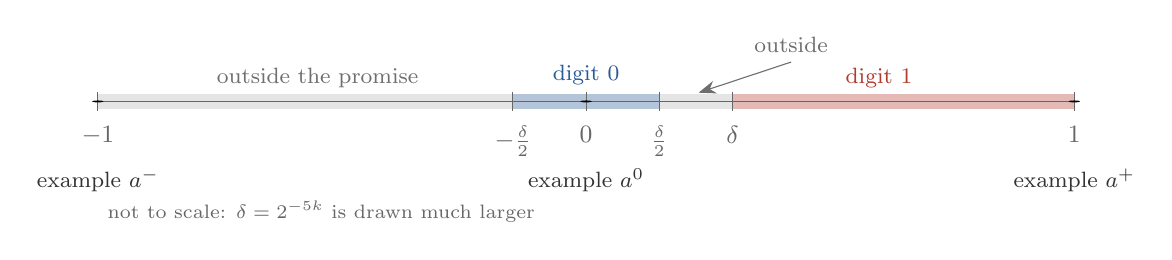
\begin{tikzpicture}[x=6.2cm, font=\small]
\def\d{0.3}
% outside the promise
\fill[lose!18] (-1,-0.09) rectangle (-\d/2,0.09);
\fill[lose!18] (\d/2,-0.09) rectangle (\d,0.09);
% digit zero and digit one
\fill[addr!35] (-\d/2,-0.09) rectangle (\d/2,0.09);
\fill[win!35] (\d,-0.09) rectangle (1,0.09);
\draw[black!60] (-1,0) -- (1,0);
\foreach \x/\l in {-1/{$-1$}, 0/{$0$}, 1/{$1$}}
  \draw[black!60] (\x,0.12) -- (\x,-0.12) node[below=2pt] {\l};
\draw[black!60] (-\d/2,0.12) -- (-\d/2,-0.12) node[below=2pt] {$-\tfrac{\delta}{2}$};
\draw[black!60] (\d/2,0.12) -- (\d/2,-0.12) node[below=2pt] {$\tfrac{\delta}{2}$};
\draw[black!60] (\d,0.12) -- (\d,-0.12) node[below=2pt] {$\delta$};
% region labels
\node[lose, font=\footnotesize] at (-0.55,0.3) {outside the promise};
\node[addr, font=\footnotesize, align=center] at (0,0.33) {digit $0$};
\node[win, font=\footnotesize] at (0.6,0.3) {digit $1$};
\draw[lose, ->, shorten >=1pt] (0.42,0.5) node[above, font=\footnotesize] {outside} -- (0.225,0.1);
% example strings
\foreach \x/\n in {-1/{a^-}, 0/{a^0}, 1/{a^+}} {
  \fill[black] (\x,0) circle[radius=0.012];
  \node[font=\footnotesize, black!80] at (\x,-1.0) {example $\n$};}
\node[font=\scriptsize, black!60, anchor=west] at (-1,-1.4) {not to scale: $\delta=2^{-5k}$ is drawn much larger};
\end{tikzpicture}
\end{document}
